\documentclass{article}
\usepackage[utf8]{inputenc}
\usepackage{authblk}
\usepackage{setspace}
\usepackage[margin=1.25in]{geometry}
\usepackage{graphicx}
\graphicspath{{./figures/}}
\usepackage{amsmath}
\usepackage{array}
\usepackage{booktabs}
\usepackage{tabularx}
\usepackage{algorithm}
\usepackage{algorithmic}
\usepackage{lineno}
\usepackage{hyperref}
\hypersetup{hidelinks}
\linenumbers

\usepackage[
style=nejm,
citestyle=numeric-comp,
sorting=none
]{biblatex}
\addbibresource{sample.bib}

\title{SARS: An Explainable Student Academic Performance Risk Assessment and Advisory System}

\author[1]{Kethavath Santhosh}
\author[1]{Jumpala Vignesh}
\author[1]{S P S Sai Suraj}
\author[2]{Dr. Sunil Bhutada}

\affil[1]{Department of Information Technology, Sreenidhi Institute of Science and Technology (SNIST), Hyderabad, Telangana, India.}
\affil[2]{Head of Department, Department of Information Technology, Sreenidhi Institute of Science and Technology (SNIST), Hyderabad, Telangana, India.}
\affil[]{\texttt{22311a12p9@sreenidhi.edu.in}, \texttt{22311a12p6@it.sreenidhi.edu.in}, \texttt{22311a12n5@it.sreenidhi.edu.in}}

\date{}

\onehalfspacing

\begin{document}

\maketitle

\begin{abstract}
Academic institutions worldwide collect detailed student performance data across multiple semesters, yet existing academic information systems serve primarily administrative purposes without providing interpretive, predictive, or actionable insights. Faculty advisors struggle to identify at-risk students early enough for effective intervention, while students lack tools to understand their academic trajectory and receive personalized guidance. Predictive systems that do exist frequently operate as black boxes, generating opaque risk scores that limit practical utility and raise transparency concerns in educational settings where trust and student agency are important.

This paper presents SARS, a Student Academic Performance Risk Assessment and Advisory System, an explainable decision-support platform designed for early academic risk detection and personalized advisory support in higher education institutions. The system makes three principal contributions: an automated grade ingestion pipeline using a multimodal document extraction workflow to convert photographs or scans of official grade sheet documents into structured academic records; a multi-factor risk scoring engine computing a SARS Score from 0 to 100 as a credits-weighted composite of GPA trend, backlog accumulation, and attendance compliance with placement policy floor rules; and an evidence-grounded advisory pipeline using ChromaDB vector storage and Gemini text-embedding-004, where student data is decomposed into typed knowledge chunks retrieved semantically per query with source citations accompanying every response. The system was validated using real grade sheet documents spanning five semesters and demonstrated across a synthetic cohort covering all four risk levels. Evaluation confirms formula accuracy, risk classification alignment with institutional policy, and effective retrieval across varied advisory question types.
\end{abstract}

\noindent\textbf{Keywords:} Educational Data Mining, Learning Analytics, Student Risk Assessment, Academic Advisory System, Decision Support Systems, Document Analysis

\section{Introduction}
Academic risk in higher education remains a persistent global challenge because dropout, prolonged degree completion, and academic failure impose substantial personal, financial, and institutional costs. Early warning systems have repeatedly shown value when intervention occurs with sufficient lead time, especially in environments where advisors can connect predictive signals to targeted support measures \cite{baker2014edm,essa2012predictive,arnold2012course}. However, much of the literature assumes digitally mature universities with continuous learning management system logs, structured clickstream traces, and course interaction data streams. Such assumptions are poorly aligned with institutions in which official academic records are still distributed through printed or scanned grade sheets, semester credit loads vary significantly, and autonomous grading frameworks follow local academic regulations rather than standardized administrative schemas.

Within autonomous higher education settings, academic risk is frequently recognized only after semester examination results are released, by which time the opportunity for timely remediation may already be reduced. This delay becomes particularly consequential near placement season, when cumulative grade point average, backlog history, and attendance thresholds determine employability and internship eligibility. Faculty advisors often lack unified cohort-level dashboards for identifying vulnerable students, while students themselves remain uncertain about placement readiness until recruitment processes are already underway. Existing prediction systems also tend to emit opaque risk scores through conventional machine learning pipelines, thereby limiting interpretability and trust in high-stakes educational decision support \cite{jayaprakash2014early,romero2020survey,khosravi2022xai}.

The SARS system is proposed to address these limitations through an end-to-end pipeline that combines three capabilities not typically found together in academic analytics platforms. First, a multimodal document extraction workflow automates grade ingestion from physical or scanned documents, reducing manual transcription effort. Second, a calibrated multi-factor risk engine computes an explainable SARS score with transparent factor contributions and institutional policy floor rules. Third, a retrieval-grounded advisory subsystem grounds natural-language guidance in retrieved student-specific evidence, returning source citations for every answer. This integration transforms raw grade sheets into actionable and auditable academic guidance rather than isolated administrative records.

The remainder of the paper is organized as follows. Section 2 reviews related work on educational early warning systems, academic performance prediction, explainable analytics, and retrieval-grounded advisory systems. Section 3 presents the materials and methods underlying the SARS design. Section 4 reports the evaluation results. Section 5 discusses practical implications and limitations. Section 6 concludes the paper and outlines future work.

\section{Related Work}
Educational Data Mining and learning analytics have established the conceptual foundation for student risk identification by transforming educational traces into predictive and intervention-oriented signals \cite{baker2014edm}. Early institutional deployments such as Rio Salado College's predictive analytics framework and Purdue University's Course Signals demonstrated that proactive alerting can improve retention and student success outcomes \cite{essa2012predictive,arnold2012course}. These systems showed that dashboards and warning indicators can shift advising from reactive to proactive practice. Nevertheless, their operating assumptions are tightly coupled to learning management system telemetry, assignment submission logs, and online engagement metrics that are not uniformly available in many autonomous or resource-constrained institutions.

Academic performance prediction research has since broadened from rule-based alerts to multi-factor analytic models. The Open Academic Analytics Initiative proposed a richer early alert framework by combining GPA, credits attempted, and completion behavior into a composite risk index \cite{jayaprakash2014early}. Broader surveys have catalogued decision trees, Bayesian models, support vector machines, neural networks, and ensemble approaches for predicting student achievement and attrition \cite{romero2020survey,hussain2019predicting,summers2021predicting}. Despite improved predictive power, a recurring limitation is that many published systems emphasize classification accuracy over operational transparency, making them difficult to deploy in advisory contexts where stakeholders must understand why a student has been flagged.

Explainable AI has therefore emerged as a central requirement in educational settings. Khosravi \emph{et al.} argue that educational AI systems must be interpretable, accountable, and aligned with pedagogical goals rather than optimized solely for prediction \cite{khosravi2022xai}. Conati \emph{et al.} similarly note that interpretable machine learning is particularly important in open-ended learning environments, where students and teachers need explanations that support reflection and decision-making \cite{conati2018interpretable}. Post-hoc techniques such as LIME and SHAP can expose feature contribution patterns, but they do not inherently provide evidence grounded in retrievable institutional records. As a result, explanations may still appear abstract to end users who need direct linkage to concrete semester results, backlog counts, or attendance history.

Large language models have expanded the scope of educational support by enabling conversational interfaces for tutoring, feedback, and advising. Foundational transformer architectures made modern embedding and generation systems possible \cite{vaswani2017attention,brown2020language}. However, standalone large language models remain susceptible to hallucination and unsupported claims, which is especially problematic in education \cite{kasneci2023chatgpt}. Retrieval-Augmented Generation was introduced to improve factual grounding by conditioning generation on retrieved external knowledge \cite{lewis2020rag}. Subsequent surveys have shown that retrieval-augmented generation can improve faithfulness, updateability, and domain adaptation across knowledge-intensive tasks \cite{gao2023rag}. Yet personalized educational advisory applications that combine student-specific retrieval, strict evidence grounding, and visible source citations remain underexplored.

Responsible deployment also requires privacy-aware design because students are sensitive to the use of academic data in analytic systems. Student perceptions of learning analytics are strongly shaped by transparency, data minimization, and perceived fairness \cite{ifenthaler2016privacy}. The gap addressed by SARS is therefore not merely predictive performance. No existing system was identified that unifies physical document digitization, calibrated multi-factor risk scoring, and citation-grounded retrieval-based advisory in a single pipeline validated on real institutional grade data. SARS positions explainability as an architectural property rather than a post-processing add-on.

\section{Materials and Methods}
\subsection{System Architecture and Methodology}
\subsubsection{Overall Architecture}
SARS follows a four-layer architecture consisting of presentation, application, data, and analytics services tiers. The presentation layer is implemented as a React 18 single-page application with role-separated student and teacher dashboards. The student interface supports profile access, grade upload, semester review, attendance submission, risk inspection, and advisory chat. The teacher interface supports cohort monitoring, student drill-down views, intervention logging, and analytics summaries. The application layer is implemented in FastAPI under Python 3.11, exposing 25 REST endpoints distributed across authentication, student, and teacher modules. This layer coordinates validation, authorization, persistence, risk recomputation, and advisory orchestration. The data layer uses SQLite with SQLAlchemy ORM and an 11-table schema supporting users, teachers, students, semester records, subject grades, attendance records, risk scores, advisory sessions, intervention logs, invite codes, audit events, and chat metadata. The analytics services layer integrates document extraction, response generation, embedding services, and ChromaDB for persistent vector retrieval.

\begin{figure}[t]
\centering
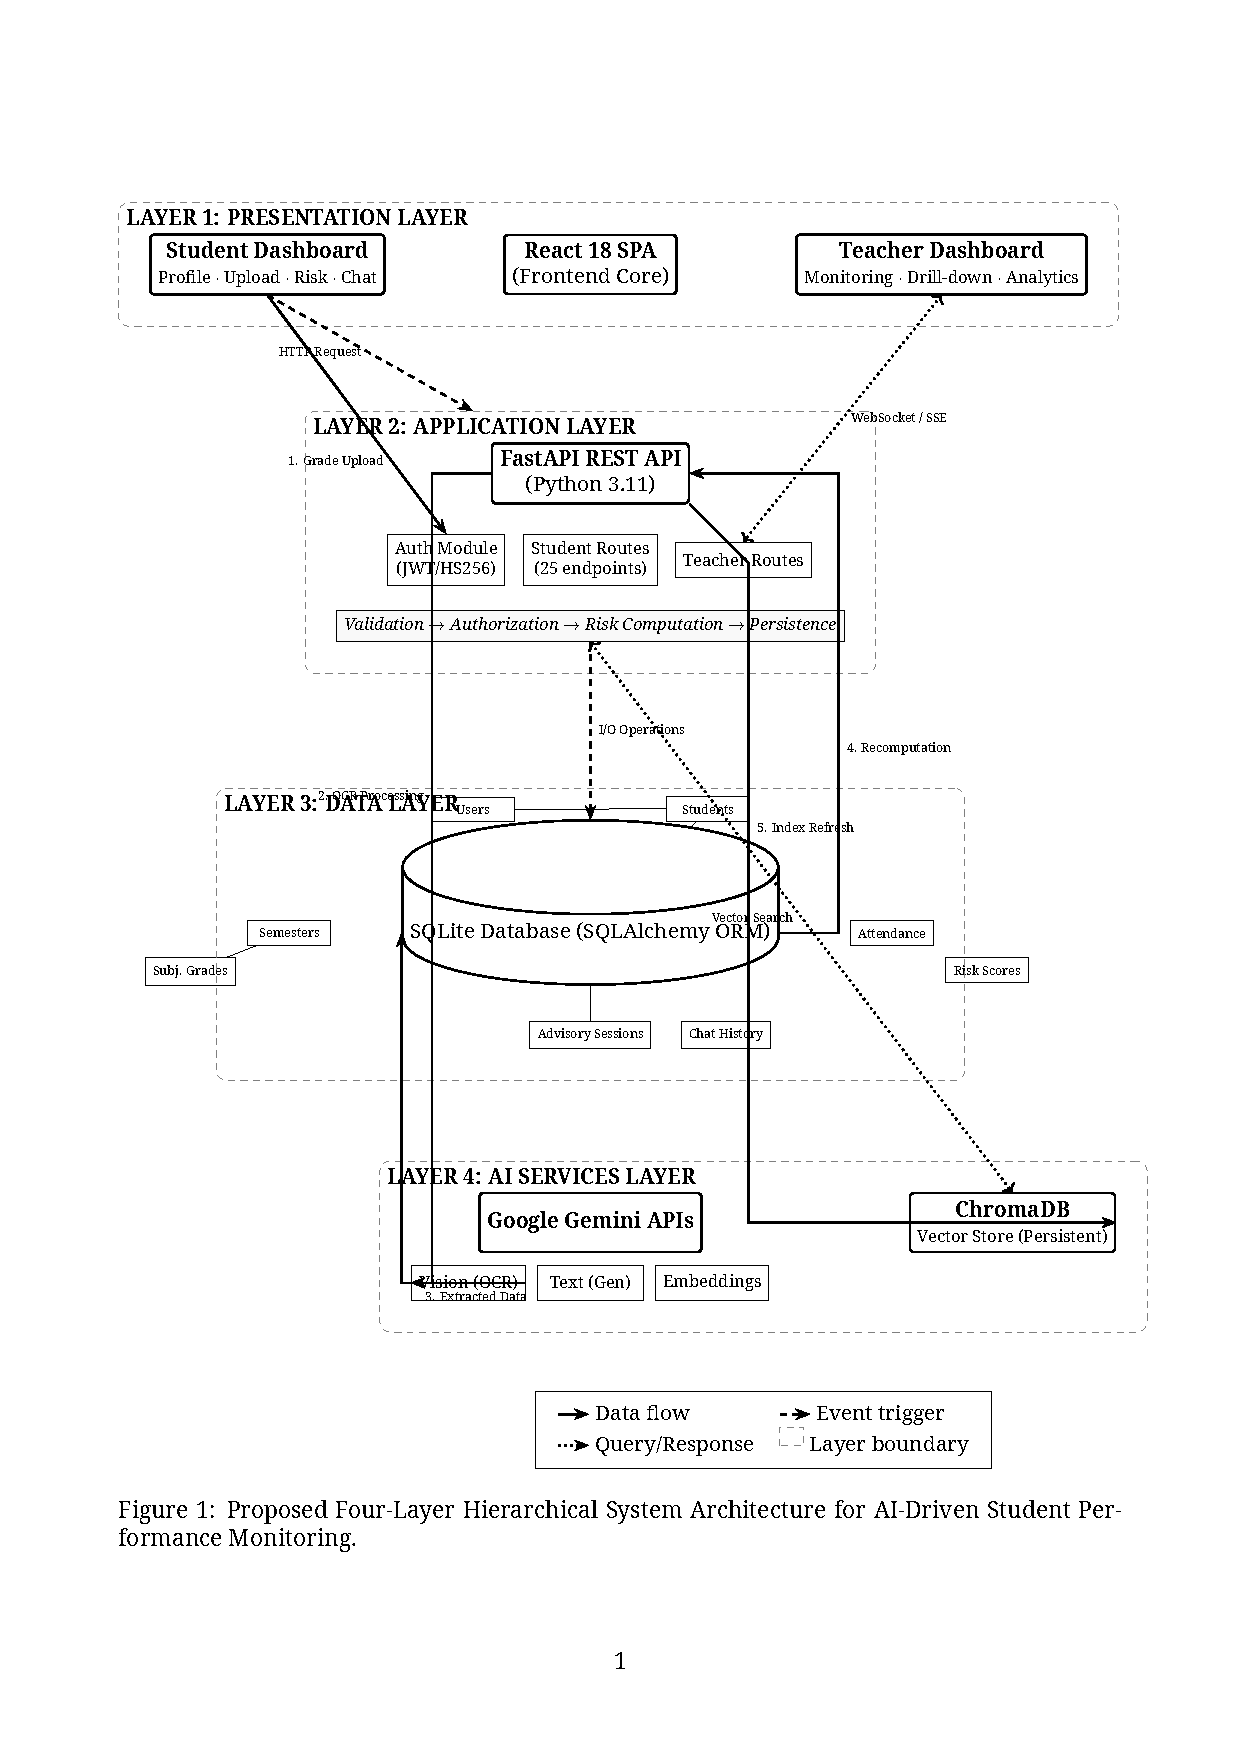
\includegraphics[width=0.92\textwidth]{system_architecture_diagram.pdf}
\caption{High-level SARS system architecture showing the separation between user-facing dashboards, transactional services, relational persistence, and analytics-support components.}
\label{fig:architecture}
\end{figure}

The grade ingestion pipeline begins when a student uploads either a PDF or an image of an official grade sheet. PDF submissions are rendered through PyMuPDF at 3$\times$ zoom, corresponding to approximately 216 DPI, in order to preserve small tabular text. Image uploads are upscaled so that the longest side is at least 2500 pixels, after which Pillow applies contrast enhancement by a factor of 1.3 and sharpness enhancement by a factor of 1.5. This preprocessing stage improves optical interpretability for compact academic tables that include subject codes, grade letters, credits, and summary statistics. The processed page is encoded as JPEG in base64 and transmitted to a multimodal extraction service; the current prototype uses Gemini 2.5 Flash Vision together with a structured prompt that explicitly requests JSON output. Extraction reliability is improved by setting \texttt{temperature = 0.1} for deterministic behavior and \texttt{max\_output\_tokens = 8192} to avoid truncation on semesters containing a large number of subjects.

The model response is parsed by stripping markdown wrappers and decoding the resulting JSON object. A normalization stage then maps grade letters onto the institutional 10-point scale, flags backlogs for grades such as F, AB, NS, and NS*, and infers the semester number from examination text when it is not directly encoded in a structured field. Before any persistence occurs, the extracted information is presented back to the student in a review form that enables manual correction. This human-in-the-loop confirmation step is important because academic records are high-stakes data artifacts. Figure~\ref{fig:extraction-review} illustrates this review stage, in which document metadata, semester aggregates, and subject-level entries remain editable before confirmation. Once confirmed, the data are written into \texttt{semester\_records} and \texttt{subject\_grades}, after which downstream triggers recompute the SARS score and refresh the vector index.

\begin{figure}[t]
\centering
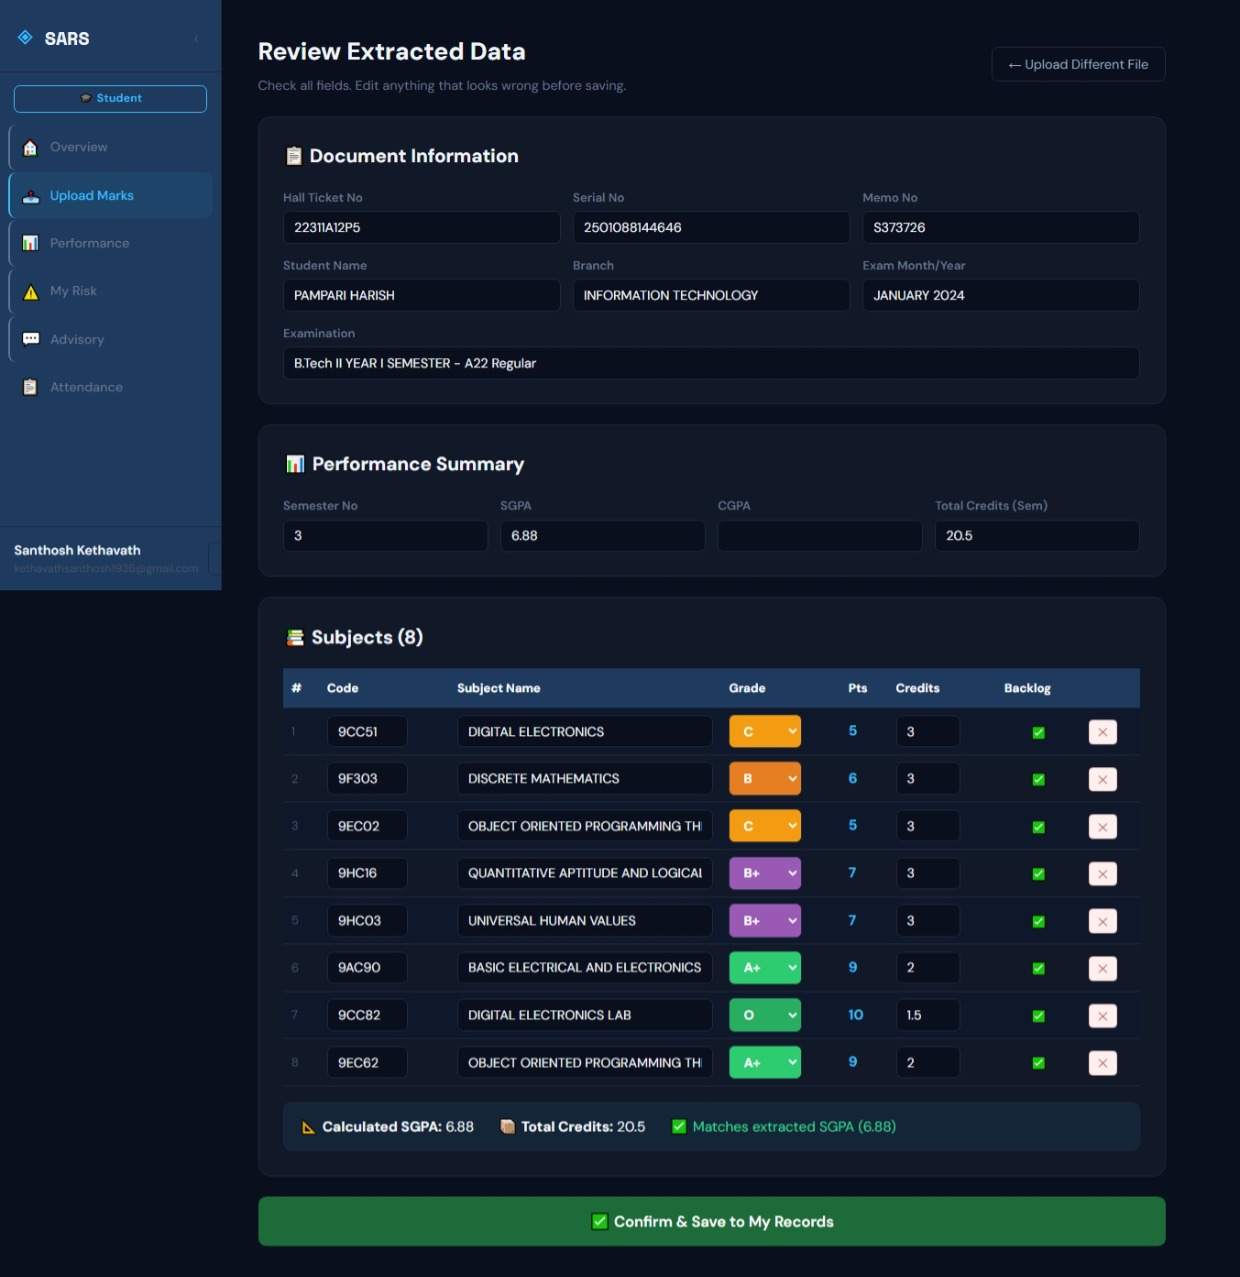
\includegraphics[width=0.96\textwidth]{extraction_review.jpeg}
\caption{Human-in-the-loop validation screen used to review and correct extracted semester data before storage.}
\label{fig:extraction-review}
\end{figure}

\begin{algorithm}[t]
\caption{Event-Driven SARS Update Pipeline}
\label{alg:update}
\begin{algorithmic}[1]
\STATE Receive student action: grade upload, semester deletion, or attendance update
\STATE Validate JWT, role, payload schema, and rate limits
\IF{uploaded artifact is PDF or image}
\STATE Preprocess document and call the extraction service for JSON output
\STATE Present extracted fields for user confirmation
\ENDIF
\STATE Persist confirmed academic data through SQLAlchemy transactions
\STATE Recompute CGPA, backlog totals, attendance summary, and SARS score
\STATE Rebuild student knowledge chunks and upsert them into ChromaDB
\STATE Mark advisory context as refreshed and return updated dashboard data
\end{algorithmic}
\end{algorithm}

\subsubsection{Security Architecture}
Because SARS stores academic records and produces advisory outputs that may influence student choices, the security model is designed to enforce both authentication and controlled disclosure. Authentication is handled through JSON Web Tokens signed with HS256 and configured with a 24-hour expiry window. Passwords are hashed with bcrypt using 12 rounds, with explicit 72-byte truncation before hashing to align with bcrypt limits and avoid edge-case incompatibilities. Role-based access control separates student and teacher capabilities at the route dependency level. Teacher registration additionally requires an administrator invite code so that elevated accounts cannot be created freely.

Operational safeguards are layered on top of the authentication core. Brute-force mitigation limits login attempts to five per minute per client IP address, while advisory chat requests are limited to ten messages per minute per student account to prevent abuse of the advisory interface. Input validation is enforced on attendance entries, grade fields, and document submission metadata. Cross-origin resource sharing is parameterized through environment variables to prevent permissive deployment defaults. A startup assertion blocks launch when the configured \texttt{SECRET\_KEY} is weak or unchanged from a default value. These measures collectively support confidentiality, integrity, and bounded resource consumption while preserving a usable advisory experience.

\subsection{SARS Risk Scoring Model}
\subsubsection{Credits-Weighted CGPA Computation}
The risk model begins with a credits-weighted cumulative grade point average calculation because semester loads are not uniform across the curriculum. Let $\mathrm{SGPA}_i$ denote the semester grade point average for semester $i$ and let $C_i$ denote the credits attempted in that semester. The cumulative grade point average is computed as
\begin{equation}
\mathrm{CGPA} = \frac{\sum_{i=1}^{n} \mathrm{SGPA}_i \cdot C_i}{\sum_{i=1}^{n} C_i}.
\label{eq:cgpa}
\end{equation}
This formulation differs from a simple arithmetic mean of semester grade point averages because it appropriately weights semesters with heavier credit loads. In autonomous programs where laboratory, project, and theory credits vary across semesters, simple averaging systematically distorts the cumulative result by overemphasizing lighter semesters and underemphasizing heavier ones. The weighted formulation therefore matches official transcript practices and serves as the correct basis for downstream risk assessment.

\subsubsection{Composite SARS Score}
The SARS score aggregates grade point average, backlog, and attendance signals into a single normalized risk value on a 0--100 scale:
\begin{equation}
\mathrm{SARS} = 0.40 \cdot R_{\mathrm{gpa}} + 0.35 \cdot R_{\mathrm{backlog}} + 0.25 \cdot R_{\mathrm{att}}.
\label{eq:sars}
\end{equation}
The grade point average risk component measures distance from the placement eligibility threshold $T_{\mathrm{placement}} = 7.5$:
\begin{equation}
R_{\mathrm{gpa}} = \max\left(0, \frac{T_{\mathrm{placement}} - \mathrm{CGPA}}{T_{\mathrm{placement}}}\right) \cdot 100.
\label{eq:gpa-risk}
\end{equation}
The attendance risk component penalizes deviation below the institutional attendance expectation:
\begin{equation}
R_{\mathrm{att}} = \max\left(0, \frac{75 - A_{\mathrm{avg}}}{75}\right) \cdot 100,
\label{eq:attendance-risk}
\end{equation}
where $A_{\mathrm{avg}}$ is the average attendance percentage across uploaded attendance records. When no attendance data are available, the system uses a conservative default of $25.0$ to reflect partial uncertainty instead of assuming perfect compliance.

Backlog risk is intentionally modeled as a non-linear penalty rather than a linear count multiplier because the marginal academic and placement impact of each additional backlog is not constant. A first backlog is a warning signal, but accumulated backlogs rapidly constrain placement eligibility, increase remediation burden, and correlate with broader academic instability. The adopted mapping is shown in Table~\ref{tab:backlog-risk}.

\begin{table}[t]
\caption{Non-Linear Backlog Risk Mapping}
\label{tab:backlog-risk}
\centering
\begin{tabular}{cc}
\toprule
Backlogs & Risk Points \\
\midrule
0 & 0 \\
1 & 40 \\
2 & 60 \\
3 & 80 \\
4 & 90 \\
5+ & 100 \\
\bottomrule
\end{tabular}
\end{table}

Temporal academic momentum is incorporated through a grade point average trend modifier. Let
\begin{equation}
\Delta = \mathrm{SGPA}_{\mathrm{latest}} - \mathrm{SGPA}_{\mathrm{previous}}.
\end{equation}
If $\Delta < -0.8$, ten points are added to $R_{\mathrm{gpa}}$ to reflect a sharp decline. If $-0.8 \leq \Delta < -0.2$, five points are added for moderate deterioration. If $\Delta > 0.5$, five points are subtracted to recognize meaningful improvement. This modifier preserves interpretability while incorporating directional change rather than treating the transcript as a static snapshot.

\subsubsection{Placement Policy Floor Rules and Classification}
To align analytics with institutional decision thresholds, the score is bounded by policy floor rules that enforce minimum risk bands when severe conditions are present. These rules prevent an apparently moderate aggregate from masking categorical disqualification conditions such as low cumulative grade point average or multiple backlogs.

\begin{table}[t]
\caption{Placement Policy Floor Rules}
\label{tab:floor-rules}
\centering
\resizebox{\textwidth}{!}{
\begin{tabular}{lll}
\toprule
Condition & Minimum Risk Level & Minimum Score \\
\midrule
CGPA $< 5.0$ & HIGH & 75 \\
$5.0 \leq$ CGPA $< 7.0$ & MODERATE & 50 \\
$7.0 \leq$ CGPA $< 7.5$ & WATCH & 25 \\
Backlogs $\geq 3$ & HIGH & 75 \\
$1 \leq$ Backlogs $\leq 2$ & MODERATE & 50 \\
\bottomrule
\end{tabular}
}
\end{table}

\begin{table}[t]
\caption{SARS Risk Level Classification}
\label{tab:risk-levels}
\centering
\resizebox{\textwidth}{!}{
\begin{tabular}{lll}
\toprule
Score Range & Level & Interpretation \\
\midrule
0--24.9 & LOW & On track \\
25.0--49.9 & WATCH & Attention needed \\
50.0--74.9 & MODERATE & Intervention recommended \\
75.0--100.0 & HIGH & Immediate action required \\
\bottomrule
\end{tabular}
}
\end{table}

The final score is translated into an ordinal risk level for dashboard visualization and advisory tone control. The model also reports a confidence score that communicates evidential completeness rather than predictive certainty. Confidence is set to $1.0$ when at least two semesters and attendance data are available, $0.75$ when at least two semesters are present but attendance is missing, $0.60$ when only one semester has been uploaded, and $0.40$ when no semester data exist. This measure prevents over-interpretation of sparse profiles and supports responsible communication of uncertainty.

\subsection{Evidence-Grounded Advisory Pipeline}
\subsubsection{Motivation for Selective Retrieval}
Naively sending the full student record, complete semester history, and prior conversation on every advisory query is inefficient and does not scale. In the SARS deployment context, such context stuffing consumes approximately 3000 tokens per request, reducing throughput and increasing cost. Selective retrieval reduces this footprint by retrieving only the most relevant evidence, lowering token usage to roughly 800 tokens per request and yielding a 60--70\% reduction in typical interactions. More importantly, retrieval introduces traceability: every answer can be linked back to concrete student data segments instead of being generated from a monolithic prompt. This design addresses reliability concerns associated with general large language model use in education \cite{kasneci2023chatgpt,lewis2020rag,gao2023rag}.

\subsubsection{Knowledge Chunking Strategy}
Student data are decomposed into seven typed chunk categories so that retrieval can target the semantic intent of each question. The chunking policy is summarized in Table~\ref{tab:chunks}. Deterministic chunk identifiers of the form \texttt{s\{student\_id\}\_\{type\}} enable idempotent upsert during re-indexing, ensuring that updates overwrite stale content rather than duplicating vectors.

\begin{table}[t]
\caption{Typed Student Knowledge Chunks Used in the Advisory Layer}
\label{tab:chunks}
\centering
\small
\begin{tabularx}{\textwidth}{lXX}
\toprule
Chunk Type & Content & Purpose \\
\midrule
identity & Name, CGPA, semester, branch, roll number summary & Profile and overview questions \\
risk\_summary & SARS score, factor breakdown, confidence, level & Risk interpretation questions \\
semester\_N & Subject-wise grades, credits, semester GPA & Specific grade and semester record questions \\
backlogs & Failed subjects, unresolved backlog counts, remediation cues & Backlog strategy and arrear planning \\
attendance & Per-subject attendance percentages and averages & Attendance compliance questions \\
cgpa\_trajectory & Semester-wise SGPA trend and progression notes & What-if and trajectory reasoning \\
placement\_eligibility & Threshold comparison, disqualifiers, readiness assessment & Placement eligibility questions \\
\bottomrule
\end{tabularx}
\normalsize
\end{table}

\subsubsection{Indexing Pipeline}
Each chunk is embedded using Gemini \texttt{text-embedding-004} with \texttt{task\_type = retrieval\_document}. The resulting vectors are stored in a persistent ChromaDB collection named \texttt{sars\_student\_knowledge}. Student-level isolation is enforced through metadata filters keyed by \texttt{student\_id}, which prevents cross-student retrieval while preserving a shared collection for operational simplicity. Re-indexing is triggered automatically whenever grade upload confirmation, semester deletion, attendance update, or risk recomputation occurs. This event-driven design makes the knowledge store self-maintaining and removes the need for manual synchronization between transactional records and retrieval context.

\subsubsection{Retrieval and Response Workflow}
At query time, the student question is embedded using the same Gemini embedding model with \texttt{task\_type = retrieval\_query}. A ChromaDB similarity search is then executed with a \texttt{student\_id} filter, returning the top four chunks for the current user. Retrieved chunks are assigned qualitative relevance labels based on vector distance: values below 0.3 are treated as HIGH relevance, values below 0.6 as MEDIUM relevance, and larger distances as LOW relevance. Only these retrieved chunks are inserted into the advisory prompt, and the response model is instructed to answer exclusively from the supplied evidence. A rolling history of the last six conversation messages is appended to preserve conversational continuity without overwhelming the prompt.

\begin{figure}[t]
\centering
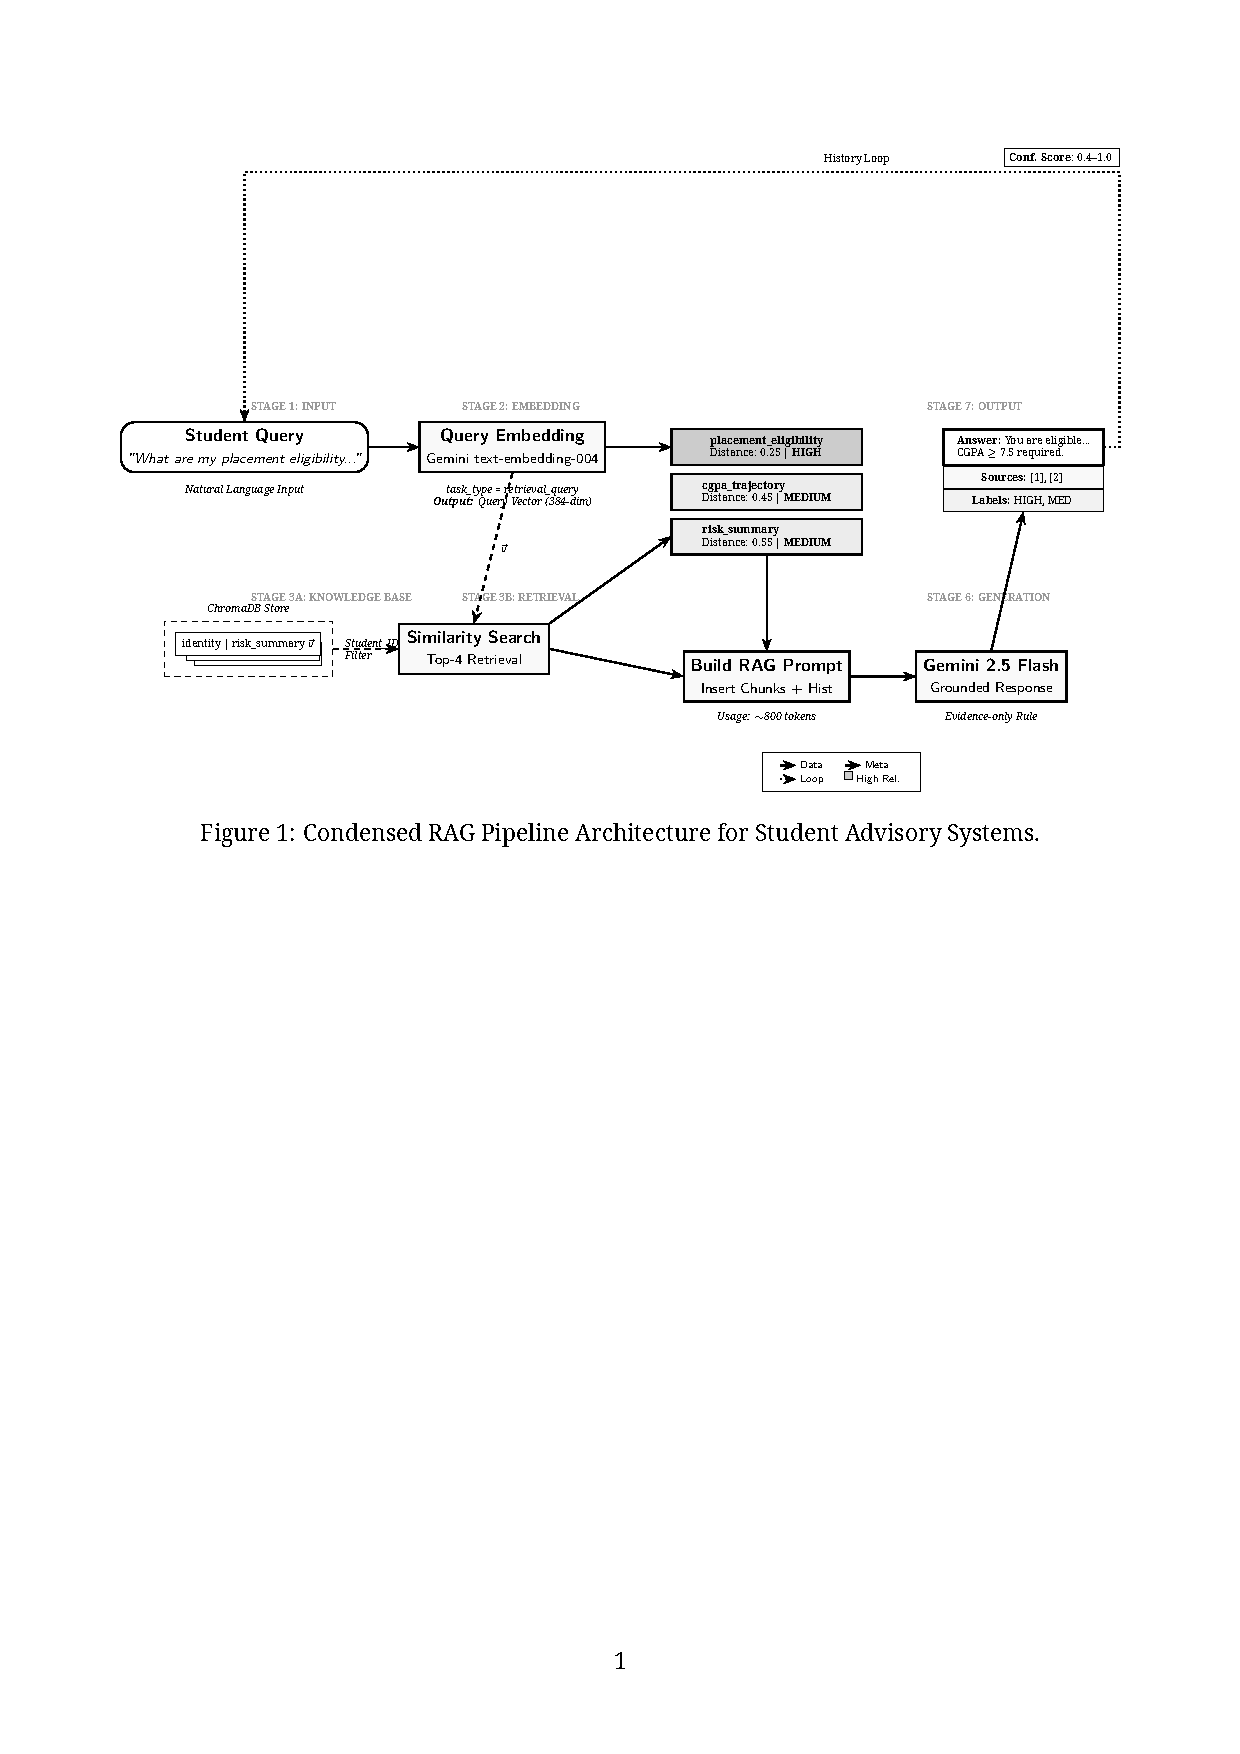
\includegraphics[width=0.92\textwidth]{rag_pipeline_diagram.pdf}
\caption{Evidence-grounded advisory pipeline in which student queries are grounded through typed retrieval before response generation.}
\label{fig:rag}
\end{figure}

The response generation service, implemented in the current prototype with Gemini 2.5 Flash, then produces a grounded natural-language answer, and the API returns both the textual response and a structured \texttt{sources} array. Each source includes the chunk type, relevance label, and a 120-character preview for display in the frontend. This enables users to inspect which evidence informed the answer, thereby converting explainability from a hidden model property into an explicit interface feature.

\subsubsection{Automation Behaviors}
Although SARS is not framed as an autonomous decision-maker, it includes three automation behaviors that reduce manual maintenance. First, indexing is automatic because confirmed data updates automatically refresh the knowledge base. Second, risk recomputation is automatic because any grade or attendance change triggers a fresh SARS score without requiring a user to request recalculation. Third, advisory context refresh is automatic because chat threads track a \texttt{data\_updated} state and force a re-index before the next answer when the current context is stale. These properties allow the system to maintain stateful coherence across academic updates while keeping human users in control of final decisions.

\section{Results}
\subsection{Grade Extraction Accuracy}
The grade extraction module was evaluated on real grade sheet documents from two students spanning seven semester uploads and 66 subjects in total. Table~\ref{tab:extraction} shows that all subjects were extracted correctly after increasing \texttt{max\_output\_tokens} from 2048 to 8192, which resolved earlier truncation failures in 11-subject semesters.

\begin{table}[t]
\caption{Grade Extraction Accuracy on Real Grade Sheets}
\label{tab:extraction}
\centering
\begin{tabular}{lcccc}
\toprule
Student & Sem. & Subjects & Extracted & Accuracy \\
\midrule
Student A & 5 & 47 & 47 & 100\% \\
Student B & 2 & 19 & 19 & 100\% \\
Total & 7 & 66 & 66 & 100\% \\
\bottomrule
\end{tabular}
\end{table}

\subsection{CGPA Formula Validation}
The correctness of the weighted cumulative grade point average formulation was tested against official records. Table~\ref{tab:cgpa-validation} shows that the credits-weighted computation exactly matched the official value, whereas a simple mean of semester grade point averages produced a slight overestimation. The discrepancy is expected because simple averaging under-weights semesters carrying heavier credit loads.

\begin{table}[t]
\caption{CGPA Formula Validation}
\label{tab:cgpa-validation}
\centering
\begin{tabular}{lccc}
\toprule
Student & Weighted CGPA & Simple Avg & Official \\
\midrule
Student A & 8.55 & 8.57 & 8.55 \\
\bottomrule
\end{tabular}
\end{table}

\subsection{Demo Cohort Risk Distribution}
To demonstrate categorical behavior across all alert levels, a synthetic cohort of eight representative students was created. The resulting distribution is shown in Table~\ref{tab:cohort}. The examples cover high-performing students, borderline placement cases, moderate-risk profiles with accumulating backlogs, and severe cases constrained by policy floor rules.

\begin{table}[t]
\caption{SARS Score Distribution Across the Demonstration Cohort}
\label{tab:cohort}
\centering
\resizebox{\textwidth}{!}{
\begin{tabular}{lcccc}
\toprule
Student Name & CGPA & Backlogs & SARS Score & Level \\
\midrule
Ravi Kumar Sharma & 9.10 & 0 & 6.3 & LOW \\
Priya Lakshmi Reddy & 8.60 & 0 & 8.1 & LOW \\
Arjun Venkata Naidu & 7.90 & 0 & 28.4 & WATCH \\
Sneha Anjali Patel & 7.30 & 0 & 29.2 & WATCH \\
Mohammed Farhan & 6.50 & 2 & 58.3 & MODERATE \\
Lakshmi Sravani Devi & 5.80 & 1 & 62.1 & MODERATE \\
Venkat Suresh Boyapati & 4.90 & 4 & 82.5 & HIGH \\
Divya Sree Krishna & 4.20 & 6 & 87.3 & HIGH \\
\bottomrule
\end{tabular}
}
\end{table}

While Table~\ref{tab:cohort} provides a controlled summary of the synthetic evaluation cohort, the deployed teacher-facing interface surfaces the same risk signals in an operational monitoring view. Figure~\ref{fig:risk-monitor} shows how faculty can scan cohort counts, inspect individual SARS scores and labels, and prioritize follow-up based on concise advisory cues.

\begin{figure}[t]
\centering
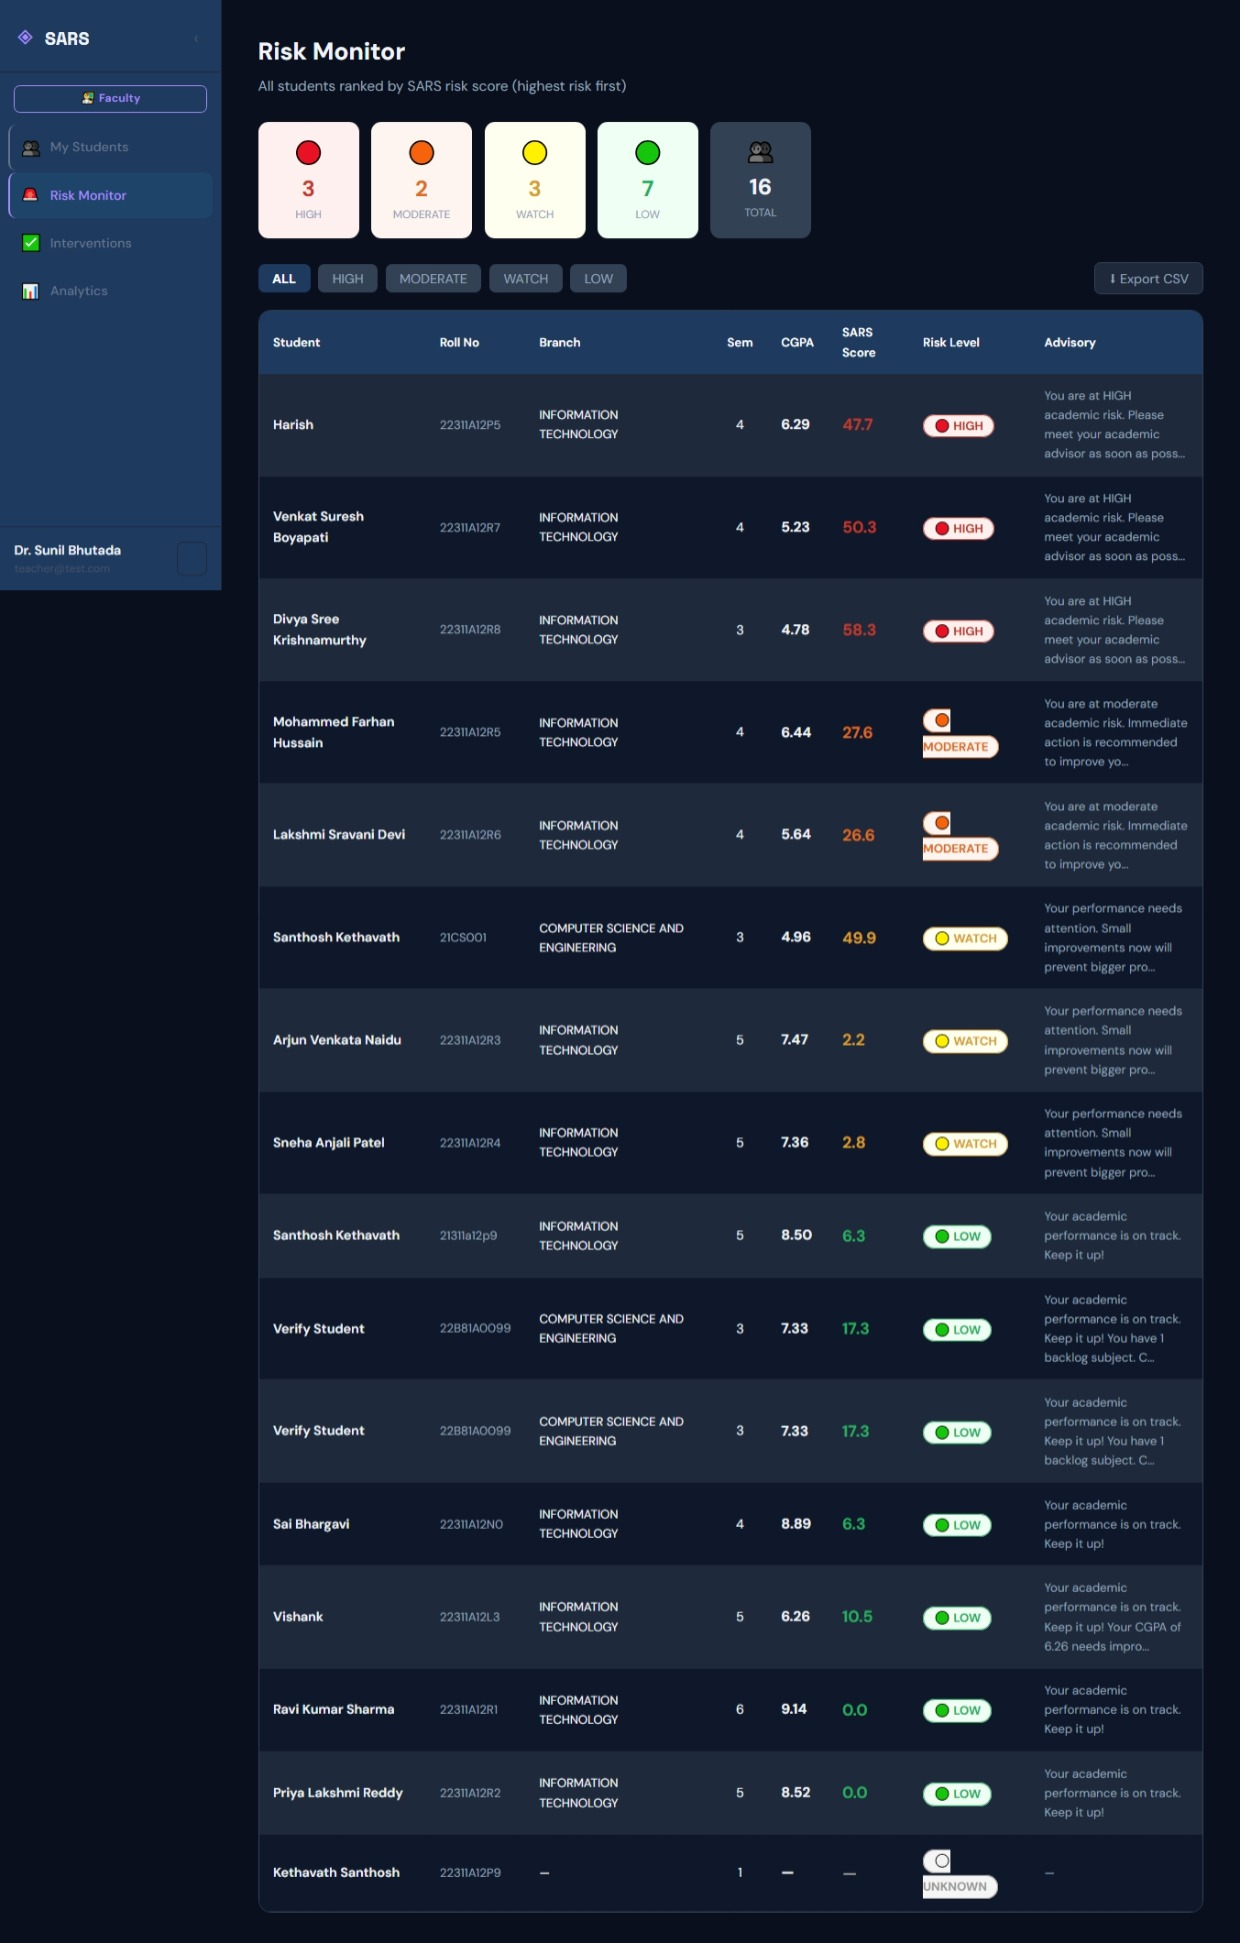
\includegraphics[width=0.96\textwidth]{risk_monitor.jpeg}
\caption{Teacher risk monitor summarizing cohort counts, per-student SARS scores, assigned risk bands, and short intervention-oriented guidance.}
\label{fig:risk-monitor}
\end{figure}

\subsection{Retrieval Evaluation}
Retrieval quality was evaluated by issuing representative questions across five advisory intents and checking whether the expected chunk class appeared among the retrieved results. Table~\ref{tab:retrieval} shows correct retrieval for all tested categories, yielding 100\% typed-query retrieval accuracy in the evaluation set.

\begin{table}[t]
\caption{Retrieval Evaluation}
\label{tab:retrieval}
\centering
\resizebox{\textwidth}{!}{
\begin{tabular}{llll}
\toprule
Question Type & Expected & Retrieved & Correct \\
\midrule
Risk level query & risk\_summary & risk\_summary & Yes \\
Specific grade query & semester\_N & semester\_N & Yes \\
Placement eligibility & placement\_eligibility & placement & Yes \\
What-if CGPA query & cgpa\_trajectory & cgpa\_traj & Yes \\
Backlog strategy & backlogs & backlogs & Yes \\
\bottomrule
\end{tabular}
}
\end{table}

\subsection{Context Efficiency}
The operational advantage of selective retrieval over context stuffing is summarized in Table~\ref{tab:tokens}. Under a 1M-token daily budget, the retrieval-based design increases service capacity by approximately 3.75$\times$ while preserving evidence grounding.

\begin{table}[t]
\caption{Context Efficiency Comparison}
\label{tab:tokens}
\centering
\begin{tabular}{lcc}
\toprule
Approach & Tokens/Request & Daily Capacity \\
\midrule
Context Stuffing & $\sim$3000 & $\sim$333 requests \\
Selective Retrieval & $\sim$800 & $\sim$1250 requests \\
Reduction & 73\% & 3.75$\times$ improvement \\
\bottomrule
\end{tabular}
\end{table}

\section{Discussion}
Several findings emerge from the evaluation. First, credits-weighted cumulative grade point average is not a minor implementation detail but a necessary condition for correctness in institutions where credit loads vary across semesters. Second, the non-linear backlog penalty better captures the practical consequences of academic arrears than a linear formulation because each additional unresolved backlog increasingly constrains placement opportunities and remediation bandwidth. Third, the retrieval layer reduces token consumption by 73\% while improving response groundedness through explicit source citations, thereby providing both efficiency and explainability.

The practical implications are significant for institutions lacking deep portal integration or learning management system centered analytics. SARS demonstrates that meaningful academic intelligence can still be constructed from scanned or photographed grade sheets through a document digitization pathway. The dual-dashboard design supports both student self-awareness and teacher oversight, enabling a shared but role-sensitive view of academic standing. By exposing the chunk sources that informed each advisory response, the system addresses the trust deficit repeatedly noted in the black-box early warning literature \cite{jayaprakash2014early,khosravi2022xai,conati2018interpretable}.

Several limitations remain. SQLite is convenient for a prototype and small deployments but is not appropriate for heavily concurrent institutional production use. The retrieval-based advisory pipeline depends on Gemini API availability, and free-tier or quota-based rate limits can constrain usage at scale. The thresholds used in the current risk engine, including the 7.5 cumulative grade point average placement cut-off and 75\% attendance expectation, are calibrated for a specific institutional context and must be recalibrated before transfer to other universities. In addition, multilingual advisory support has not yet been implemented, and longitudinal validation across multiple cohorts and institutions has not been completed. These observations align with broader cautions in educational analytics and machine learning deployment research \cite{hussain2019predicting,summers2021predicting}.

Responsible deployment considerations are central to the deployment stance adopted by SARS. Advisory outputs are framed as analytic guidance rather than deterministic predictions so that student agency is preserved. The retrieval layer is designed around typed academic summaries and metadata filters rather than indiscriminate exposure of personally identifiable information. Confidence values are surfaced alongside risk scores to communicate uncertainty and data completeness. Teacher access restrictions, invite-code controls, and privacy-aware data handling reflect the importance of transparency and bounded access in learning analytics environments \cite{ifenthaler2016privacy,khosravi2022xai}.

\section{Conclusion and Future Work}
This paper presented SARS, an end-to-end academic risk assessment and advisory system that combines three complementary contributions: multimodal grade digitization from physical academic documents, an explainable multi-factor risk engine, and a citation-grounded retrieval-based advisory layer. Evaluation demonstrated 100\% extraction accuracy on real grade sheets, correct cumulative grade point average computation matching official records, risk classifications aligned with placement policy, and a 73\% token reduction for retrieval-based advisory relative to context stuffing. The overall architecture supports both student self-monitoring and faculty intervention, while embedding explainability directly into the user experience through factor breakdowns and cited evidence.

Future work includes migration to PostgreSQL for production-scale concurrency, workflow-based what-if planning for multi-step student scenarios, attendance extraction from attendance sheets using the same document processing pipeline, multi-language advisory support for regional languages, longitudinal validation across multiple institutions and cohorts, integration with institutional student information systems through REST connectors, and a mobile application for direct camera capture and upload. These extensions would broaden the operational scope of SARS while preserving the core principle that academic analytics should remain transparent, contextual, and actionable.

\section*{Acknowledgments}
The authors gratefully acknowledge the academic guidance of Dr. Sunil Bhutada and the institutional support of Sreenidhi Institute of Science and Technology, Hyderabad.

\printbibliography

\end{document}
